
\subsection{Punto 1}

Analizar que función cumple y como opera el subcircuito compuesto por $R_{12}$ a $R_{17}$, $C_{16}$ y $U_{3}A$. Luego incluir $R_{S}$. ¿Qué características tiene éste subcircuito, por ejemplo, su transferencia, su ancho de banda, su dependencia de las especificaciones del amplificador operacional $TL082$, de sus fuentes de alimentación, de la temperatura, de la tolerancia y tecnología de los resistores con los que se lo implemente, etc.

\clearpage

\subsection{Punto 2}

 Analizar qué función cumple y como opera el subcircuito compuesto por $R_{18}$ a $R_{19}$, $C_{15}$ y $U_{3}B$. ¿Qué características tiene éste subcircuito, por ejemplo, su transferencia, su ancho de banda, su dependencia de las especificaciones del amplificador operacional $TL082$, de sus fuentes de alimentación, de la temperatura, de la tolerancia y tecnología de los resistores con lo que se lo implemente, etc. ($R_{18}$ puede variarse desde $0 \Omega$ a $18 K\Omega$).

\clearpage

\subsection{Punto 3}

Analizar qué función cumple y cómo opera el subcircuito compuesto por $R_{20}$ a $R_{23}$ y $Q_{7}$-$Q_{9}$-$Q_{10}$-$Q_{11}$. ¿Qué características tiene éste subcircuito?

\clearpage

\subsection{Punto 4}

Analizar el subcircuito que proporciona la tensión de referencia. ¿Cómo funciona y qué características tiene? Por ejemplo: hallar por cálculo y por simulación el valor de la tensión de referencia y su dependencia de la variación de la tensión de entrada $V_{1}$, de la temperatura ambiente y de la corriente que pueda entregar éste subcircuito a otros subcircuitos que alimente. Consultar las hojas de datos de todos sus componentes, en especial el $TL431$.

\clearpage

\subsection{Punto 5}

Analizar el subcircuito compuesto por $Q_{4}$ y $Q_{5}$. Por ejemplo: con que nombre es conocida su topología, comprobar si es una topología que emplea realimentación, qué características funcionales tiene este subcircuito, que valores de impedancia presente a los otros circuitos que alimente, cual es la transferencia de este subcircuito (variable de salida / variable de entrada), cuál es su ancho de banda, etc.

\clearpage

\subsection{Punto 6}

¿Cuál es el rango de la tensión de salida de la fuente considerando que $R_{9}$ puede variar desde $0 \Omega$ a $90 K\Omega$? (Tomar $R_{L} = 1M\Omega$).

\clearpage

\subsection{Punto 7}

¿Cuál es el rango la corriente de salida de la fuente considerando que $R_{18}$ puede variar desde $0 \Omega$ a $18 K\Omega$? (Tomar $R_{L} = 0\Omega$).

\clearpage

\subsection{Punto 8}

¿Cuál es el valor de la resistencia de carga $R_{L}$ que impone el límite entre el modo fuente de tensión y fuente de corriente para $R_{9} = 90 K\Omega$ y $R_{18} = 0 \Omega$?.

\clearpage

\subsection{Punto 9}

¿Qué hace (o para que está) cada componente, o sea, que función cumple en el circuito y justificar el valor de cada resistencia, diodo, transistor, etc?\\
En particular, respecto de la pregunta anterior, explicar que función realiza $D_{1}$ y justificar la elección de su designación como $1N4148$.

\clearpage

\subsection{Punto 10}

¿Qué tecnología, tolerancia, capacidad de disipación de potencia, estabilidad con la temperatura, tensión y corriente de operación máxima y pulsante, características mecánicas, apartamiento de su valor nominal por envejecimiento, etc, debe tener cada componente considerando una implementación física de éste circuito?.

\clearpage

\subsection{Punto 11}

Calcular la ganancia de lazo \quotemarks{af} para el lazo de tensión y para el lazo de corriente, comparando en ambos casos con respecto a 1, o sea, ¿Resulta \quotemarks{af} mucho mayor que $1$? Considerar esto para frecuencias del orden de entre $0 Hz$ y $100 Hz$.

\clearpage

\subsection{Punto 12}

Calcular la impedancia de salida, o más propiamente la impedancia en el nodo de salida, para una carga de $100 \Omega$ y una frecuencia en el entorno a $50Hz$. Utilizar para el cálculo los mismo modelos utilizados en la pregunta anterior.

\clearpage

\subsection{Punto 13}

Hallar por simulación la impedancia del nodo de salida en función de la frecuencia para frecuencias desde $0,1 Hz$ hasta $100 KHz$ y con $R_{L} = 100 \Omega$. Considerar $R_{9} = 10 K\Omega$.

\clearpage

\subsection{Punto 14}

Hallar por simulación la impedancia de la malla de salida en función de la frecuencia para frecuencias desde $0,1 Hz$ hasta $100 KHz$ y con  $R_{L} = 0 \Omega$. Considerar  $R_{18} = 0 \Omega$.

\clearpage

\subsection{Punto 15}

Hallar por simulación la tensión del nodo de salida en función de la corriente de salida para  $R_{L}$ variando entre  $100 \Omega$ y $0 \Omega$. Considerar $R_{9} = 10 K\Omega$ y $R_{18} = 0 \Omega$.

\clearpage

\subsection{Punto 16}

\textbf{Enunciado}: \textsl{Hallar por simulación la variación de la tensión de salida en función del tiempo para un salto abrupto de la corriente de salida desde aproximadamente $0 A$ hasta $ 1A$ y posteriormente un salto abrupto de la corriente de salida desde aproximadamente $ 1A$ hasta $0 A$. Considerar $R_{9} = 10 K\Omega$ y $R_{18} = 0 \Omega$.}


\vspace{1.5cm}


Para lograr la conmutación de la carga se utilizó el circuito mostrado en la figura~\figref{fig:fig_p16_rl_switch}, donde se puede ver el modelo de una llave controlada por tensión con resistencia de $0 \si[per-mode=symbol]{\ohm}$ en estado cerrado y resistencia tendiendo a infinito (valor muy grande) para el estado abierto. El switch es controlado por una onda cuadrada, de tal manera de lograr una carga de $0 \si[per-mode=symbol]{\ampere}$ al comienzo de la simulación, de $1 \si[per-mode=symbol]{\ampere}$ ($R_{L} = 2 \si[per-mode=symbol]{\ohm}$) a los $20 \si[per-mode=symbol]{\milli\second}$, y luego nuevamente $0 \si[per-mode=symbol]{\ampere}$ a los $50 \si[per-mode=symbol]{\milli\second}$. La simulación realizada es del tipo transitorio (\textbf{SPICE} \textit{.tran}), la salida de la misma se muestra resaltando el momento de las transiciones en la figura~\figref{fig:fig_p16_output_in_load_jump}. En la figura~\figref{fig:fig_p16_output_variation_in_load_jump} se destaca la diferencia en la tensión de salida en carga respecto a en vacío, esta diferencia permite estimar la resistencia de salida de la fuente de alimentación, el valor obtenido es:\\


\begin{equation}
R_{o} = \frac{\Delta V}{\Delta I} = \frac{\num{3.67E-4} \si[per-mode=symbol]{\volt}}{1.0137 \si[per-mode=symbol]{\ampere}} = 642 \si[per-mode=symbol]{\micro\ohm}
\end{equation}

\begin{figure}[H] %htb
\begin{center}
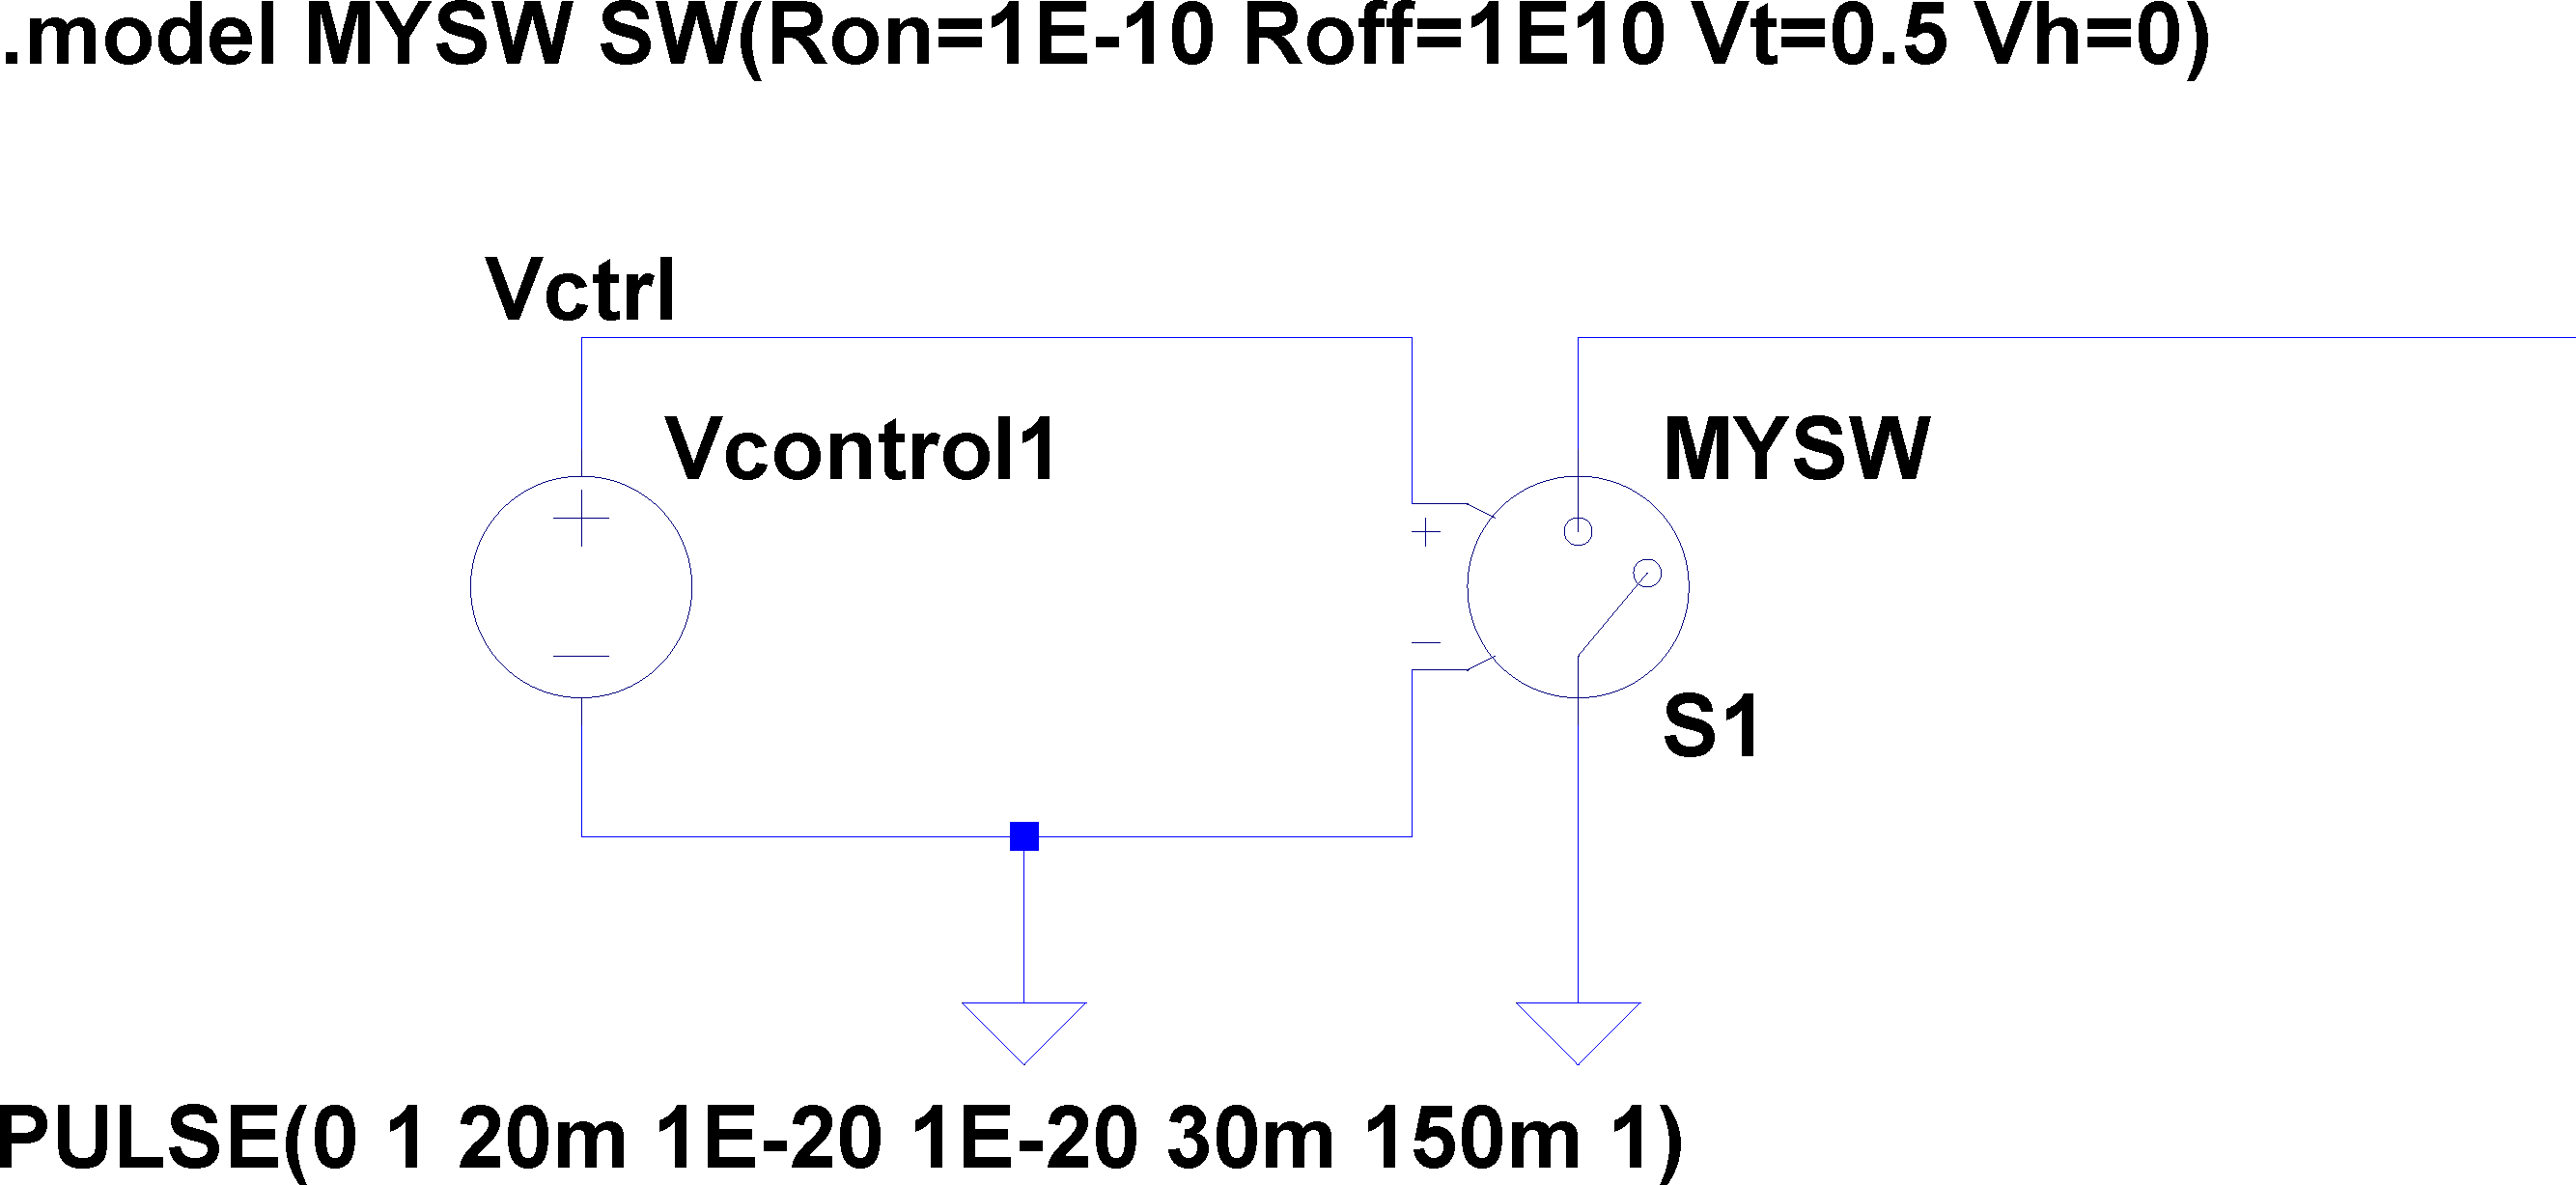
\includegraphics[width=0.9 \textwidth, angle=0]{./img/preguntas/p16a.png}
\caption{\label{fig:fig_p16_rl_switch}\footnotesize{Circuito usado para la conmutación de la carga}}
\end{center}
\end{figure}


\vfill

\clearpage

\begin{figure}[H] %htb
\begin{center}
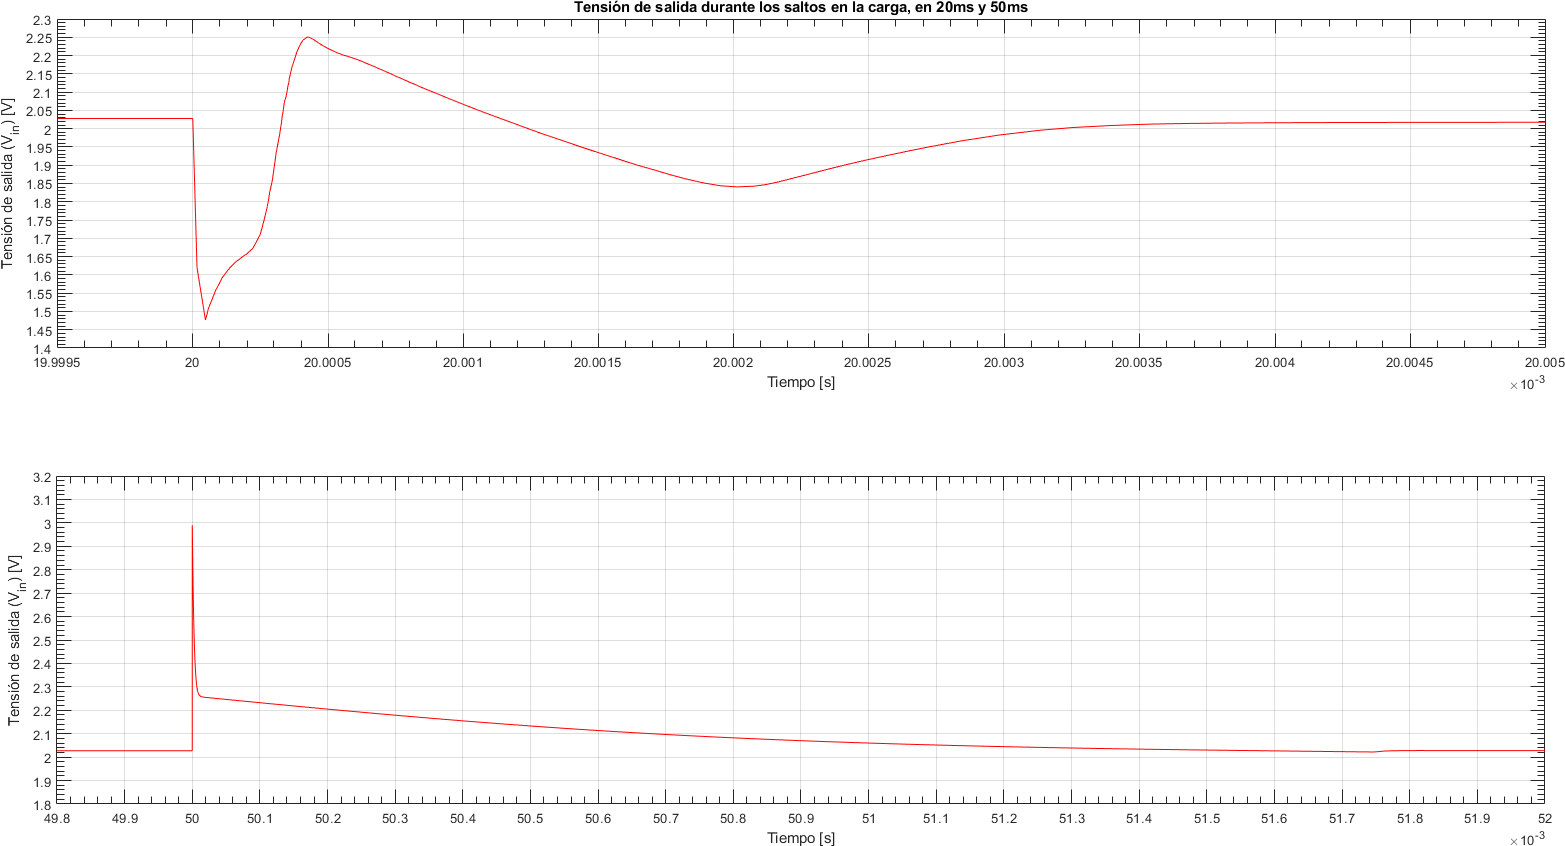
\includegraphics[width=1.2 \textwidth, angle=90]{./img/preguntas/p16b.png}
\caption{\label{fig:fig_p16_output_in_load_jump}\footnotesize{Tensión de salida frente a saltos de carga de $0 \si[per-mode=symbol]{\ampere}$ a $1 \si[per-mode=symbol]{\ampere}$ y de $1 \si[per-mode=symbol]{\ampere}$ a $0 \si[per-mode=symbol]{\ampere}$.}}
\end{center}
\end{figure}


\clearpage

\begin{figure}[H] %htb
\begin{center}
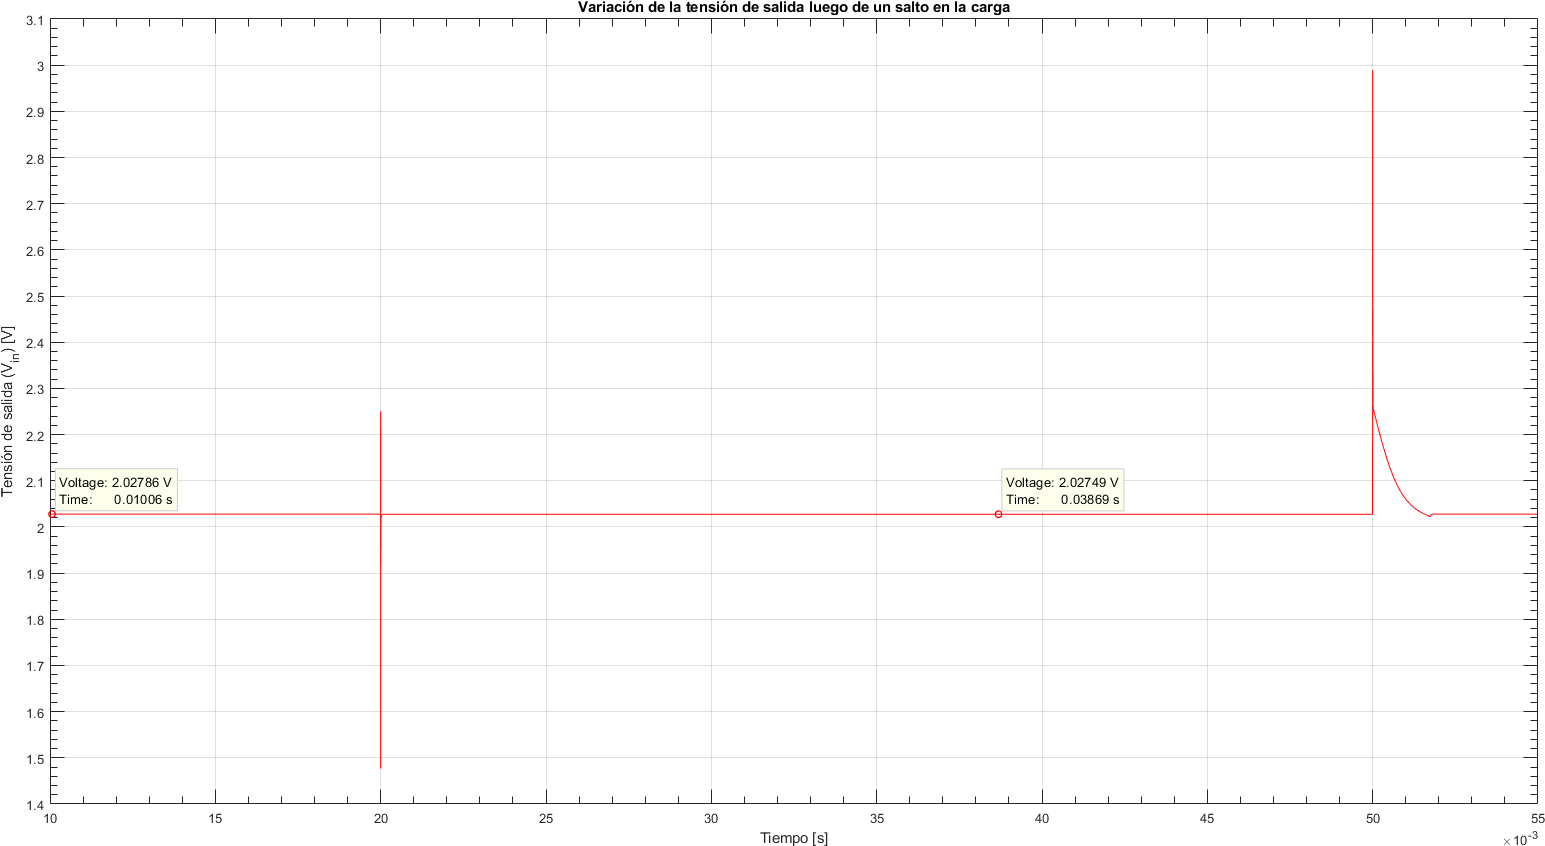
\includegraphics[width=1.2 \textwidth, angle=90]{./img/preguntas/p16c.png}
\caption{\label{fig:fig_p16_output_variation_in_load_jump}\footnotesize{Variación de la tensión de salida en los saltos de carga}}
\end{center}
\end{figure}




\clearpage


\subsection{Punto 17}

\textbf{Enunciado}: \textsl{Calcular la eficiencia para $V_{1}$ igual a $15 V$, $20 V$ y $25 V$.}

\begin{enumerate}
\item[\textsl{a)}] \textsl{con} $R_{L} = 10 \Omega$, $R_{9} = 90 K\Omega$ y $R_{18} = 0 \Omega$.
\item[\textsl{b)}] \textsl{con} $R_{L} = 1 \Omega$, $R_{9} = 0 \Omega$ y $R_{18} = 0 \Omega$.
\end{enumerate}


\vspace{1.5cm}

Para calcular la eficiencia de la fuente de alimentación simplemente se aplicó la definición $\eta = \frac{P_{out}}{P_{in}}$, el cálculo se realizó en estado estacionario, ignorando el consumo durante los transitorios, los cuales de todas formas, a largo plazo, deben ser despreciables. El cálculo se realizó directamente dentro del \textbf{LTSPICE}, utilizando el comando de \textbf{SPICE}, \textit{.measure}, este comando permite realizar cálculos utilizando valores de variables simuladas, y luego operar con estos resultados. Realizando una simulación de \textbf{SPICE} de punto de operación, \textit{.op}, se realizan las siguientes mediciones:

%******************************************************************************************
\lstset{language=,xleftmargin=1em,numbers=none}

\lstset{showspaces=false}
\lstset{showstringspaces=false}
\normalfont
\normalsize
\lstset{backgroundcolor=\color{white},rulecolor=\color{blue}}
\lstset{basicstyle=\ttfamily\color{Deepblue}}

\lstset{keywordstyle=[1]\ttfamily\color{red}\bfseries}
\lstset{keywordstyle=[2]\ttfamily\color{LightSkyBlue}}
\lstset{keywordstyle=[3]\ttfamily\bfseries\color{Plum}}
\lstset{keywordstyle=[4]\ttfamily\bfseries\color{Chocolate}}

\lstset{identifierstyle=\ttfamily\color{black}}
\lstset{commentstyle=\ttfamily\color{blue}\textit}
\lstset{stringstyle=\ttfamily\color{purple}\upshape}
\lstset{tabsize=4}

\lstset{numberstyle=\ttfamily\color{Deeppurple}\upshape}
\lstset{numbersep=5pt}

\lstset{inputencoding=utf8/latin1}



\fontencoding{T1}
\fontseries{m}
\fontsize{10pt}{11pt}
\selectfont
%******************************************************************************************


\begin{lstlisting}
.op

.meas Pin PARAM V(Vin)*(-I(V1))
.meas Pout PARAM V(Vout)*(-I(RL))
.meas Eff PARAM Pout / Pin
\end{lstlisting}



Los resultados obtenidos para la eficiencia para cada uno de los valores de tensión de entrada para la que se realizó la simulación, se resumen en la tabla~\tableref{table:table_efficiency}. Se puede ver claramente como la eficiencia disminuye al aumentar la diferencia entre la tensión de entrada y la tensión de salida, cosa totalmente esperable, ya que, a tensión de salida constante, la tensión en el elemento de paso es cada vez mayor, a la misma corriente de carga, se tiene mayor potencia disipada en el mismo.\\
También la eficiencia empeora con el aumento de la carga, ya que al pasar la corriente de carga por el elemento de paso. se disipará también mas potencia en este.\\

%% \noindent
%% \begin{center}
 
%%\begin{spacing}{1}  
\bgroup
\begin{table}[H]  %%\centering
    
    \setlength\arrayrulewidth{1.5pt}
    \arrayrulecolor{white}
    \def\clinecolor{\hhline{|>{\arrayrulecolor{white}}-%
    >{\arrayrulecolor{white}}|-|-|-|-|}}
\resizebox{0.9 \textwidth}{!}{% 
       
\def\arraystretch{2.5}
\begin{tabularx}{1 \textwidth}%
    {|
    >{\columncolor{white} \centering\arraybackslash}m{0.25\linewidth}
     |
    >{\columncolor{white} \centering\arraybackslash}m{0.25\linewidth}
     |
    >{\columncolor{white} \centering\arraybackslash}m{0.25\linewidth}
     |
    >{\columncolor{white} \centering\arraybackslash}m{0.25\linewidth}
     |
    }
    \rowcolor{HeadersColor} \cellcolor{white} \thead{}  & \thead{$V_{i} = 15 \si[per-mode=symbol]{\volt}$} & \thead{$V_{i} = 20 \si[per-mode=symbol]{\volt}$} & \thead{$V_{i} = 25 \si[per-mode=symbol]{\volt}$} \\
    
    \hhline{|-|-|-|-|}
    \rowcolor{gray!20} \cellcolor{gray!60} \thead{ \cellcolor{gray!60} $\eta = \frac{P_{out}}{P_{in}} \cdot 100 \%$ \\ \cellcolor{gray!60} \\ \cellcolor{gray!60} $R_{L} = 10 \si[per-mode=symbol]{\ohm}$, $R_{9} = 90 \si[per-mode=symbol]{\kilo\ohm}$ \\ \cellcolor{gray!60} $R_{18} = 0 \si[per-mode=symbol]{\ohm}$ } & 63.93 \% & 48.04 \% & 38.50 \%  \\
    \hhline{|-|-|-|-|}
    \rowcolor{gray!20} \cellcolor{gray!60}  \thead{ \cellcolor{gray!60} $\eta = \frac{P_{out}}{P_{in}} \cdot 100 \%$ \\ \cellcolor{gray!60} \\ \cellcolor{gray!60} $R_{L} = 1 \si[per-mode=symbol]{\ohm}$, $R_{9} = 0 \si[per-mode=symbol]{\ohm}$ \\ \cellcolor{gray!60} $R_{18} = 0 \si[per-mode=symbol]{\ohm}$ } & 6.58 \% & 4.95 \% & 3.96 \%  \\
    \hhline{|-|-|-|-|}        
    \end{tabularx}}
	\caption{\footnotesize{Eficiencia en función de la tensión de entrada.}}
	\label{table:table_efficiency}
\end{table}
\egroup
%%\end{spacing}

%% \end{center}



\clearpage

\subsection{Punto 18}

\textbf{Enunciado}: \textsl{¿Cómo influye en la tensión de salida la variación de la fuente de entrada $V_{1}$ (variando de $1 V$ a $30 V$ y con $R_{L} = 10 \Omega$, $R_{9} = 90 K\Omega$ y $R_{18} = 0 \Omega$)?. Simular para graficar la tensión de salida en función de $V_{1}$.}\\


\vspace{1.5cm}

Es de esperarse que la fuente tenga un valor mínimo de tensión de entrada, a partir del cual empieza a regular la salida, para valores menores de tensión que este valor mínimo, la salida será menor a la esperada, en principio, el regulador paralelo para regular a $10 \si[per-mode=symbol]{\volt}$, necesita una tensión de entrada mayor, pero también se deben polarizar correctamente los transistores, y como puede verse en la figura~\figref{fig:fig_p18_vo_vs_vi}, el crecimiento de la salida es prácticamente lineal, manteniendo una diferencia de aproximadamente $2.2 \si[per-mode=symbol]{\volt}$ a la salida con respecto a la entrada, este valor sería el \quotemarks{drop-out} de esta fuente de alimentación. Tomando que la salida está regulando al 
llegar a aproximadamente al $1 \%$ de la tensión regulada esperada a la salida, $10 \si[per-mode=symbol]{\volt}$, el valor de tensión de entrada mínimo para salida regulada es de $12.38 \si[per-mode=symbol]{\volt}$. También puede observarse que para tensiones muy pequeñas a la entrada, hasta aproximadamente $1.8 \si[per-mode=symbol]{\volt}$, la tensión a la salida es prácticamente $0 \si[per-mode=symbol]{\volt}$, esto se explica por estar cortado el elemento de paso de la fuente de alimentación, el par compuesto.

\vfill

\clearpage

\begin{figure}[H] %htb
\begin{center}
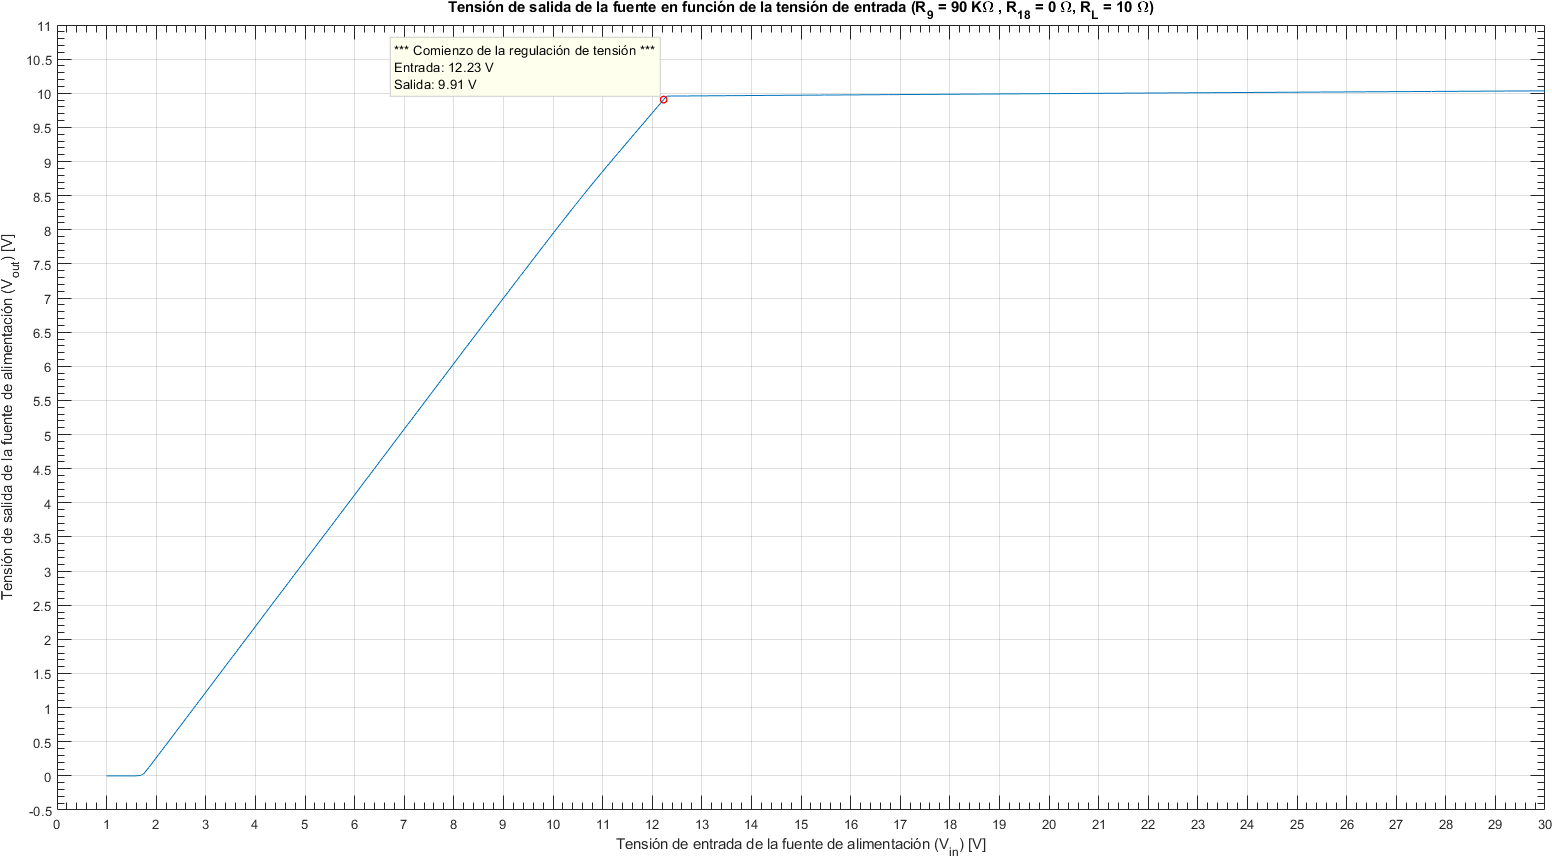
\includegraphics[width=1.2 \textwidth, angle=90]{./img/preguntas/p18.png}
\caption{\label{fig:fig_p18_vo_vs_vi}\footnotesize{Tensión de salida vs tensión de entrada.}}
\end{center}
\end{figure}

\clearpage


\subsection{Punto 19}

\textbf{Enunciado}: \textsl{¿Cómo influye en la corriente de salida la variación de la fuente de entrada $V_{1}$ (variando de $1 V$ a $30 V$ y con $R_{L} = 0 \Omega$, $R_{9} = 90 K\Omega$ y $R_{18} = 0 \Omega$?. Simular para graficar la corriente de salida en función de $V_{1}$.}\\

\vspace{1.5cm}

De la misma forma que el punto anterior, es de esperarse que la fuente tenga un valor mínimo de tensión de entrada, a partir del cual empieza a regular la salida, para valores menores de tensión que este valor mínimo, la corriente de salida será solo limitada a algún valor menor al esperado, y como puede verse en la figura~\figref{fig:fig_p19_io_vs_vi}, el crecimiento de la salida es prácticamente lineal, salvo que se produce un pico de corriente alrededor de los $3 \si[per-mode=symbol]{\volt}$ de entrada, que es limitado por la acción de $Q_{15}$, a ese valor de tensión de entrada el lazo de corriente seguramente no actúa de ninguna forma para limitar la corriente de salida. Tomando que la salida está regulando al llegar a aproximadamente al $1 \%$ de la corriente regulada esperada a la salida, $2.05 \si[per-mode=symbol]{\ampere}$, el valor de tensión de entrada mínimo para salida regulada es de $12.19 \si[per-mode=symbol]{\volt}$, valor muy cercano al del punto anterior. También puede observarse que para tensiones muy pequeñas a la entrada, aproximadamente $1.8 \si[per-mode=symbol]{\volt}$, la corriente a la salida es prácticamente $0 A$, esto se explica por la misma razón que en el punto anterior.

\vfill

\clearpage

\begin{figure}[H] %htb
\begin{center}
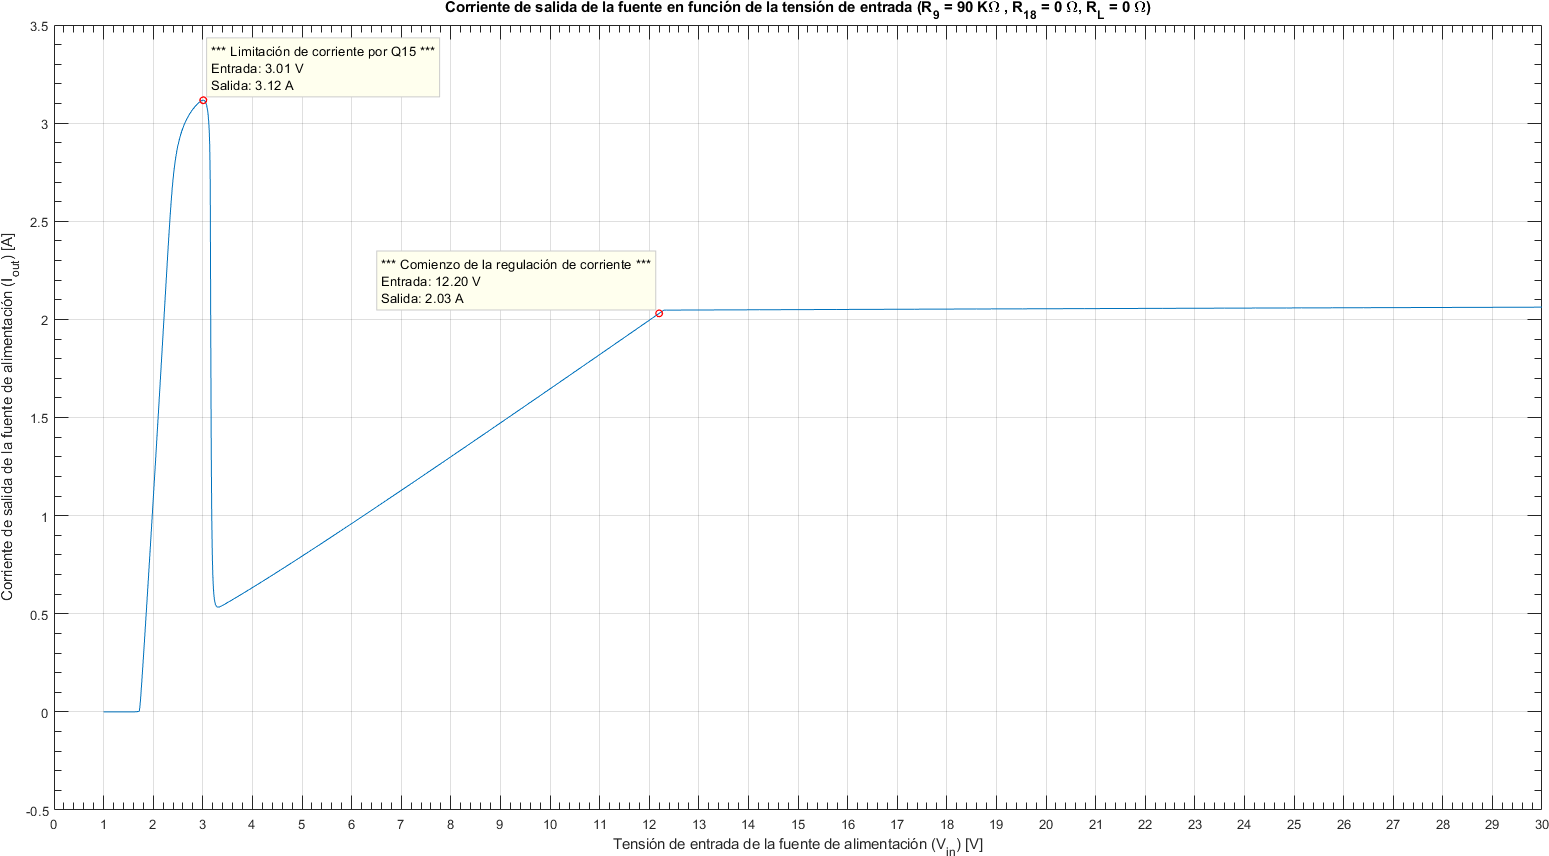
\includegraphics[width=1.2 \textwidth, angle=90]{./img/preguntas/p19.png}
\caption{\label{fig:fig_p19_io_vs_vi}\footnotesize{Tensión de salida vs tensión de entrada.}}
\end{center}
\end{figure}

\clearpage


\subsection{Punto 20}

\textbf{Enunciado}: \textsl{Determinar el rechazo de ruido, o sea, ¿Cuántos decibles de diferencia se miden comparando un ruido presente en la tensión de entrada V1 respecto del residuo de ese ruido en la tensión de salida. Debe intentarse no considerar el ruido propio de la fuente. \textbf{NOTA}: el ruido podría ser por ejemplo el rizado resultante de una rectificación y filtrado.}\\



Para ver el rechazo de ruido que presenta la fuente de alimentación, sumamos a la tensión de entrada una señal en forma de diente de sierra descendente de $100 Hz$, ya que la sugerencia era que el ruido podría provenir del rizado resultante de una rectificación y filtrado. Se utilizó una señal de $2 V$ de amplitud para poder apreciar bien la amplitud de la señal en la salida. Se graficó la entrada y la salida restándole la tensión continua de base, $20 V$ a la entrada y el valor mínimo a la salida, alrededor de $2 V$, se utilizó un script de \textbf{MATLAB} para restar los valores adecuados, hacer los cálculos y producir los gráficos a partir de los datos exportados del \textbf{LTSPICE}. En la figura~\figref{fig:fig_p20_ripple}, se muestra lo obtenido, mostrando simultáneamente 2 ciclos del rizado de entrada y salida.
Como se observa en la figura, la salida presenta un cierto tiempo de crecimiento debido al ancho de banda limitado del amplificador de la fuente, y presenta además un pequeño pico en la discontinuidad, el mismo se debe al tipo de compensación del circuito, tema que veremos en la siguiente parte del trabajo práctico. Si se mide el rechazo de ruido simplemente como el cociente de valor RMS de la señal de salida respecto de la entrada obtenemos:


\begin{equation}
    R_{nr}= 59.49 dB
\end{equation}

Sin embargo se pedía intentar no considerar el ruido propio de la fuente, entonces lo que se hizo fue, extrapolar la amplitud máxima de la señal de rizado a la salida, ignorando el sobre-pico y el tiempo de crecimiento, midiendo su amplitud cerca de la mitad de la amplitud máxima de la señal de entrada, calculado así, obtuvimos:


\begin{equation}
    R_{nr}= 61.41 dB
\end{equation}

\vfill

\clearpage

\begin{figure}[H] %htb
\begin{center}
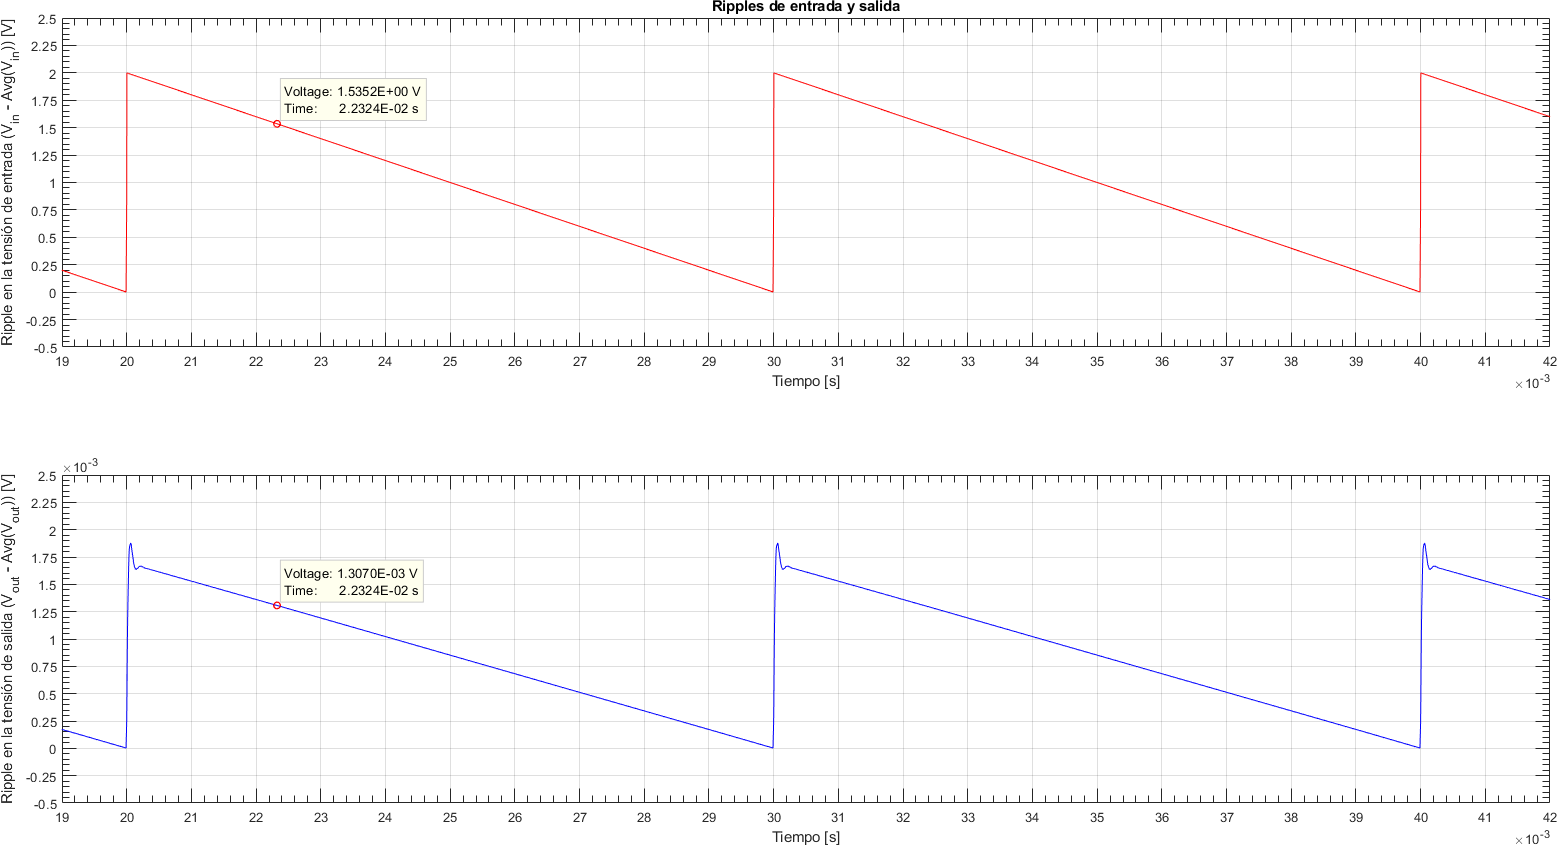
\includegraphics[width=1.2 \textwidth, angle=90]{./img/preguntas/p20.png}
\caption{\label{fig:fig_p20_ripple}\footnotesize{Rizado de entrada y salida.}}
\end{center}
\end{figure}

\clearpage


\clearpage

\subsection{Punto 21}

Modificar el circuito de la fuente reemplazando en parte o totalmente el amplificador por el regulador integrado $LM723$ y evaluar el comportamiento del nuevo diseño comparándolo con el original.

\clearpage


